\documentclass[12pt]{article}
\usepackage[utf8]{inputenc}
\usepackage{hyperref}
\usepackage{listings}
\usepackage{xcolor}
\usepackage{geometry}
\usepackage{graphicx} % For including graphics
\usepackage{minted} % For advanced code listings
\usepackage{listings-solidity}  % Include Solidity highlighting
\usepackage{amsmath, amssymb, amsfonts} % For mathematical equations


% Define a custom minted style (optional)
\usemintedstyle{colorful} % You can choose from various styles like 'monokai', 'tango', 'colorful', etc.

% Custom color setup
\definecolor{bashtextcolor}{RGB}{0, 0, 0} % Define black color

% Define a new command for inline code using minted
\newcommand{\codeinline}[1]{\mintinline{text}{#1}}

\geometry{a4paper, margin=1in}

\title{Smart Contracts Exercise 07: \\ Out of Gas}
\author{}
\date{}

% Define a new command for inline code with a dark background
\newcommand{\codeblack}[1]{%
  \texttt{\colorbox{black!7}{\textcolor{black}{#1}}}%
}

% Define a new command for inline code with a dark background
\newcommand{\codegrey}[1]{%
  \texttt{\colorbox{black!4}{\textcolor{black}{#1}}}%
}

% Define custom colors (optional)
\definecolor{myURLColor}{RGB}{0, 102, 204} % Example: A shade of blue

\hypersetup{
    colorlinks=true,        % Enable colored links
    linkcolor=blue,         % Color for internal links (e.g., \ref, \cite)
    citecolor=blue,         % Color for citations
    filecolor=magenta,      % Color for file links
    urlcolor=myURLColor     % Color for external URLs
}

% Define a style for code listings
\lstdefinestyle{mystyle}{
    backgroundcolor=\color{lightgray!20},   
    commentstyle=\color{green!50!black},
    keywordstyle=\color{blue},
    numberstyle=\tiny\color{gray},
    stringstyle=\color{red},
    basicstyle=\ttfamily\footnotesize,
    breakatwhitespace=false,         
    breaklines=true,                 
    captionpos=b,                    
    keepspaces=true,                 
    numbers=left,                    
    numbersep=5pt,                  
    showspaces=false,                
    showstringspaces=false,
    showtabs=false,                  
    tabsize=2
}

\lstset{style=mystyle}
% Adding package for header and footer
\usepackage{fancyhdr}
\pagestyle{fancy}

% Define header and footer
\fancyhf{} % Clear current settings
\fancyhead[L]{Smart Contracts Exercise 07} % Left header
\fancyhead[R]{\thepage} % Right header with page number

\renewcommand{\headrulewidth}{0.4pt} % Line below header
% \renewcommand{\footrulewidth}{0.4pt} % Line above footer

\begin{document}

\maketitle
\section{Introduction}

Oracles are essential components in decentralized applications that require external data. In this exercise, you will become familiar with both synchronous and asynchronous types of oracles, learn about the concept of decentralized exchanges, and understand their use as on-chain oracles. Finally, you will practically implement a price oracle manipulation attack using a flash loan. This will be by far the most challenging exercise in the series, with many new concepts introduced, so buckle up!

\subsection*{Project Setup}

You have two options for working with this exercise. Using docker container or local installation. Choose the one that best fits your preferences.

\subsection{Using Docker with VS Code}

This option uses Docker to create a development environment with all the necessary tools and dependencies pre-installed.

\subsubsection*{Prerequisites:}

\begin{itemize}
    \item \textbf{\href{https://www.docker.com/products/docker-desktop}{Docker}} - A platform for developing, shipping, and running applications in containers.
    \item \textbf{\href{https://code.visualstudio.com/}{Visual Studio Code}} - A lightweight but powerful source code editor.
    \item \textbf{\href{https://marketplace.visualstudio.com/items?itemName=ms-vscode-remote.remote-containers}{Dev Containers}} - An extension to VS Code that lets you use a Docker container as a full-featured development environment.
\end{itemize}

\subsubsection*{Setting Up the Project:}

\begin{enumerate}
  \item Visit the following \href{https://gitlab.fel.cvut.cz/radovluk/smart-contracts-exercises/-/tree/main/05-Re-Entrancy/task/task-code}{GitLab repository} and clone it to your local machine.
  \item Open the repository folder in VS Code.
  \item When prompted, click "Reopen in Container" or use the command palette (F1) and run \codegrey{Dev Containers: Reopen in Container}.
\end{enumerate}

\subsection{Local Setup}

If you prefer working directly on your machine without Docker, you can set up the development environment locally.

\subsubsection*{Prerequisites}
\begin{itemize}
    \item \textbf{Node.js} - \url{https://nodejs.org/en/} - An open-source, cross-platform, back-end JavaScript runtime environment that runs on the V8 engine and executes JavaScript code outside a web browser.
    \item \textbf{NPM}: Node Package Manager, which comes with Node.js.
\end{itemize}

\noindent
Open your terminal and run the following commands to verify the installations:

\begin{minted}[bgcolor=gray!5, fontsize=\footnotesize]{bash}
$ node -v
$ npm -v
\end{minted}

Both commands should return the installed version numbers of Node.js and NPM respectively. Node.js provides the runtime environment required to execute JavaScript-based tools like Hardhat, while NPM is used to manage the packages and dependencies needed for development.

\subsubsection*{Setting Up the Project}

\begin{enumerate}
    \item Visit the following \href{https://gitlab.fel.cvut.cz/radovluk/smart-contracts-exercises/-/tree/main/05-Re-Entrancy/task/task-code}{GitLab repository} and clone it to your local machine.
    \item Open a terminal and navigate to the project directory.
    \item Install the project dependencies by running \codegrey{npm install}.
\end{enumerate}

\section{Oracles}
Smart contracts cannot access data outside the blockchain on their own. They lack HTTP or similar network methods to access external sources. This is intentional to prevent non-deterministic behavior once a function is called. The blockchain does not have an internet connection! However, various Dapp applications often need external information, such as lending platforms, insurance contracts, betting contracts, wrapped cryptocurrencies, synthetics, and others. Whenever a smart contract relies on external data to compute future states, an oracle pattern is required. The disadvantages of oracles include the cost in terms of gas consumption and the risk of dependence on third parties in terms of data manipulation and data availability.

\subsection*{Synchronous Oracles}

In our example, we illustrate a situation where Alice wants to borrow USDC tokens using ETH as collateral. The problem is that the ETH/USDC price is volatile, and we need to know the current price. In a synchronous oracle, external data is periodically pushed into the oracle contract from an oracle controller. The smart contract that needs this external data—in our example, the lending platform—simply trusts that the data in the oracle smart contract is genuine and updated regularly. Look closely at the illustration in Figure \ref{fig:synchronous-oracles}. % and the simplified code example below.

\begin{figure}[h!]
  \makebox[\textwidth][ch!]{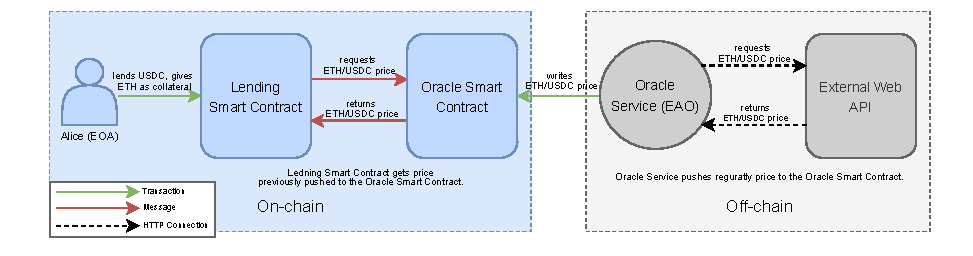
\includegraphics[width=1.1\textwidth]{synchronous_oracle.pdf}}
  \caption{Synchronous Oracles}
  \label{fig:synchronous-oracles}
\end{figure}

% Maybe not needed?
% \begin{lstlisting}[language=Solidity]
%   contract SimpleSynchronousOracle {
%     // Stored ETH/USDC price
%     int256 public price;
%     // Oracle controller service address
%     address public oracleService;
    
%     modifier onlyController() {
%         require(msg.sender == oracleService, "Not the oracle service");
%         _;
%     }
%     constructor() {
%         oracleService = msg.sender;
%     }
%     // Controller should periodically update the price
%     function updatePrice(int256 _price) public onlyController {
%         price = _price;
%     }
%     // Returns the latest price
%     function getLatestPrice() public view returns (int256) {
%         return price;
%     }
% }
% \end{lstlisting}

\subsection*{Asynchronous Oracles}

An asynchronous oracle provides data in a separate transaction after an initial request. A smart contract requests data from the oracle, which then emits an event. The oracle service fetches the data from an API or another off-chain source and subsequently sends the data back to the contract in a separate transaction.

\begin{figure}[h!]
  \makebox[\textwidth][ch!]{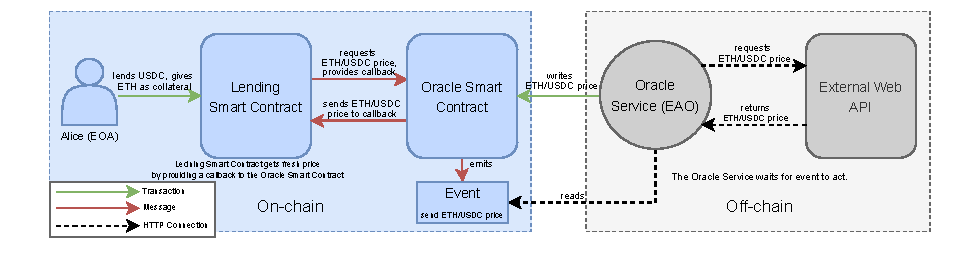
\includegraphics[width=1.1\textwidth]{asynchronous_oracle.pdf}}
  \caption{Asynchronous Oracles}
  \label{fig:asynchronous-oracles}
\end{figure}

\subsection*{DEXes as Price Oracles}

DEXes like \href{https://app.uniswap.org/}{Uniswap} or \href{https://www.sushi.com/ethereum/swap}{SushiSwap} can serve as price on-chain price oracles because they contain pools of tokens with real-time price information determined by market forces. For example, an ETH/USDC pool on a DEX can be queried to determine the current market price of ETH in USDC. More about DEXes and AMMs is provided in the next section.

\newpage
\section{Automated Market Makers}

Imagine you want to exchange your valuable token for another token or buy or sell some token with ETH. The service you are looking for is an exchange. Traditional centralized exchanges use order books where buyers and sellers are matched. Examples of such centralized services include Binance, Coinbase, Kraken etc. However, the web3 world is about decentralization, right? What if we told you that you could exchange your assets simply with a smart contract? Decentralized Exchanges (DEXes) often use Automated Market Makers (AMMs), which are smart contracts that create markets for any pair of tokens by using liquidity pools. They rely on a mathematical formula to price assets instead of using an order book. The most commonly used formula is the \textbf{Constant Product}, which follows the equation:

% \begin{figure}[H]
% \centering
% \includegraphics[width=0.9\textwidth]{dex_amm.pdf}
% \caption{Automated Market Maker Structure}
% \label{fig:amm}
% \end{figure}


\begin{equation}
  x \cdot y = k
\end{equation}

where \( x \) is the quantity of Token A in the liquidity pool, \( y \) is the quantity of Token B in the liquidity pool, and \( k \) is a constant, representing the pool's total liquidity.

\subsubsection*{Token Swaps}
When a trader swaps Token A for Token B, the new balance in the pool must still satisfy the constant product equation. If a trader adds \( \Delta x \) amount of Token A, the new state of the pool must satisfy:

\begin{equation}
    (x + \Delta x) (y - \Delta y) = k
\end{equation}

Solving for \( \Delta y \), the amount of Token B the trader receives:

\begin{equation}
    \Delta y = \frac{y \cdot \Delta x}{x + \Delta x}
\end{equation}

\subsubsection*{Price Impact}
The price of Token A in terms of Token B is given by the derivative of the invariant function:

\begin{equation}
    \frac{dy}{dx} = -\frac{y}{x}
\end{equation}

This means that as more of Token A is purchased, its price increases due to the decreasing reserve, illustrating \textbf{slippage}.

\subsubsection*{Liquidity Providers}
Liquidity Providers are individuals who deposit tokens into AMM pools. In return for their deposits, they receive special liquidity provider (LP) tokens that represent their share of the pool. To incentivize liquidity providers, a fee \( f \) (e.g., 0.3\%) is applied to each trade. This means the value of their LP tokens increases with every trade. Liquidity Providers can withdraw their liquidity and collect the accumulated fees at any time. The modified constant product formula with fees is:

\begin{equation}
  (x + \Delta x \cdot (1 - f))(y - \Delta y) = k
\end{equation}

For example, with a 0.3\% fee, the effective input amount of the trader is reduced to 99.7\% of the actual input. This can be represented as:

\begin{equation}
  (x + \Delta x \cdot 0.997)(y - \Delta y) = k
\end{equation}

Solving for \( \Delta y \), the amount of Token B the trader receives:

\begin{equation}
    \Delta y = \frac{y \cdot \Delta x \cdot 0.997}{x + \Delta x \cdot 0.997}
\end{equation}


\subsubsection*{Slippage}
A key characteristic of AMMs is that the larger the trade relative to the pool size, the more significant the price impact or "slippage." This is because removing a larger percentage of one token from the pool causes the price to move more dramatically according to the constant product formula.

\medskip
\noindent
\textbf{Tip:} Video explanation \href{https://www.youtube.com/watch?v=cizLhxSKrAc&t=2s}{How do LIQUIDITY POOLS work?}

% \begin{figure}[H]
% \centering
% \includegraphics[width=0.7\textwidth]{slippage.pdf}
% \caption{Price Slippage in AMMs}
% \label{fig:slippage}
% \end{figure}


\subsection*{Stablecoins and USDC}

Stablecoins are cryptocurrencies designed to maintain a stable value relative to a specific asset, typically a fiat currency like the US dollar. They aim to combine the benefits of cryptocurrencies (fast transfers, programmability, global accessibility) with the stability of traditional currencies.

USDC is one of the most widely-used stablecoins in the crypto ecosystem. It is simply an ERC20 token. Each USDC token should be backed by \$1 held in reserve. Circle, the company behind USDC, is regulated and publishes monthly attestations verifying these reserves. See \href{https://etherscan.io/token/0xa0b86991c6218b36c1d19d4a2e9eb0ce3606eb48}{USDC token contract on Etherscan}.

\medskip
\noindent
To learn more about DEXes, oracles and stablecoins we recommend Berkeley RDI Center on Decentralization \& AI course Decentralized Finance:
\begin{itemize}
\item \href{https://www.youtube.com/playlist?list=PLS01nW3RtgopoR-FHiMwfoMLT-opXlfJF}{DeFi MOOC Lecture 5: DEX}
\item \href{https://www.youtube.com/playlist?list=PLS01nW3RtgopICEFsRCvT_SIjoOtGa869}{DeFi MOOC Lecture 7: Stablecoins}
\item \href{https://www.youtube.com/playlist?list=PLS01nW3Rtgoo70DT2YsBmNUol4134S9C9}{DeFi MOOC Lecture 8: Oracles}
\item \href{https://rdi.berkeley.edu/berkeley-defi/f24}{The full DeFi MOOC course with materials}
\end{itemize}

\section{Task}

\subsection*{Task 1: Fool the Oracle 01}

The new rare NFT collection "FEL students" is finally on the market! The first three unique pieces are now available: Sleep-deprived OI student learning from skripta for 5000 USD, BIO pulling-all-nighter female student addicted to energy drinks for 8000 USD, and Caffeinated KYR student who will graduate only thanks to ChatGPT for 3000 USD. They are so unique and cool! You must have them all! Unfortunately, as a student, you can't afford them and start with only 3000 USDC tokens and 0.8 ETH, which is barely enough for the Caffeinated KYR student. Your goal, however, is to get them all!

\begin{figure}[h!]
  \centering
  \begin{minipage}{0.3\textwidth}
    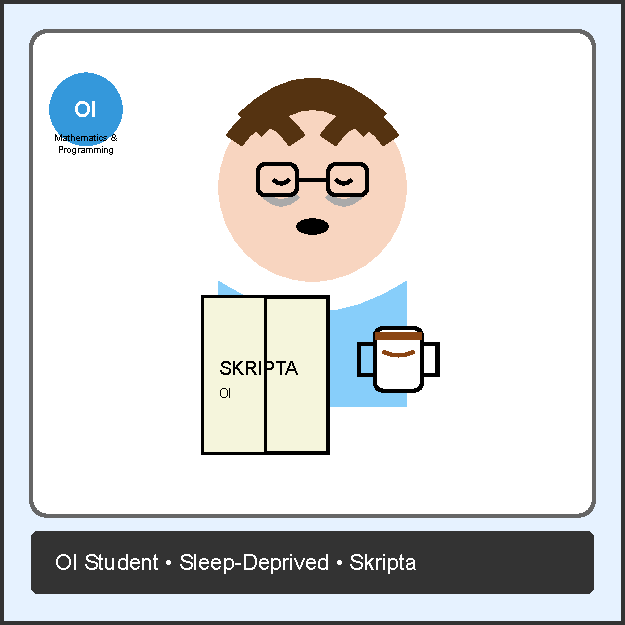
\includegraphics[width=\textwidth]{NFTs/nft-sleep-deprived-io.pdf}
  \end{minipage}
  \hfill
  \begin{minipage}{0.3\textwidth}
    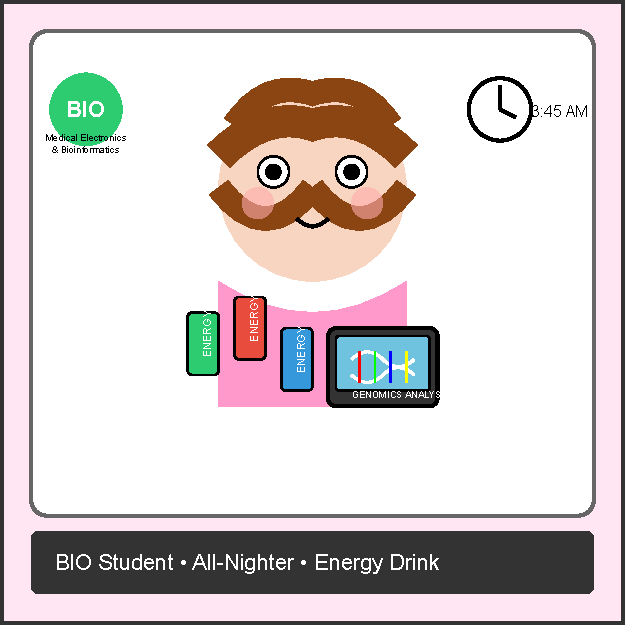
\includegraphics[width=\textwidth]{NFTs/nft-bio-pulling-allnighter.pdf}
  \end{minipage}
  \hfill
  \begin{minipage}{0.3\textwidth}
    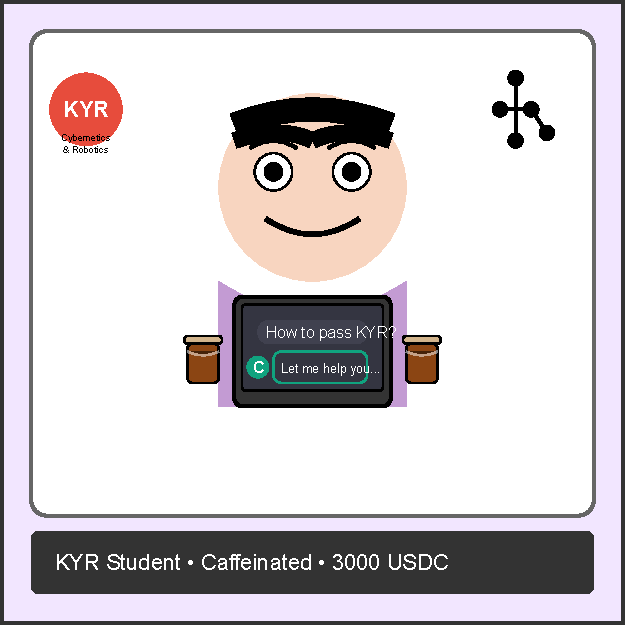
\includegraphics[width=\textwidth]{NFTs/nft-caffeinated-kyr.pdf}
  \end{minipage}
\end{figure}

\medskip
\noindent
\textbf{Your Mission:} : Buy all three NFTs that are listed on the market

\noindent
Files that are relevant for this challenge:

\begin{itemize}
\item test/\textbf{FoolTheOracle01.js}: The test file where you should code your solution.
\item contracts/\textbf{SimpleDEX.sol}: A decentralized exchange with a one liquidity pool containing 1 ETH and 2000 USDC.
\item contracts/\textbf{FELStudentNFT.sol}: A collection of unique CTU FEL Student NFTs with different traits.
\item contracts/\textbf{NFTMarketplace.sol}: A marketplace for trading these NFTs. It uses SimpleDEX as its price oracle to convert USD prices to ETH.
\item contracts/\textbf{USDCToken.sol}: An ERC20 token representing simplified version of USDC.
\end{itemize}

\noindent
Code your solution in the \texttt{test/FoolTheOracle01.js} file. Use only the player account. Verify your solution by running the following command:

\begin{minted}[bgcolor=gray!5, fontsize=\footnotesize]{bash}
  $ npm run oracle01
\end{minted}

\subsection*{Flash Loans}

Flash loans are a unique DeFi primitive that allows users to borrow assets without collateral, as long as the borrowed amount (plus any fees) is returned within the same transaction. If the borrower fails to repay, the entire transaction is reverted, ensuring lenders never lose funds. This atomic property makes flash loans a powerful tool for arbitrage, collateral swaps, and other complex DeFi operations—but also creates potential for oracle manipulation attacks. Flash loans leverage Ethereum's transaction atomicity—either the entire transaction succeeds or it fails completely. The process follows these steps:

\begin{enumerate}
    \item A user calls a flash loan provider to borrow tokens
    \item The provider transfers tokens to the user
    \item The user executes operations with the borrowed funds
    \item The user returns the borrowed amount plus fees
    \item If repayment fails, the entire transaction reverts
\end{enumerate}

This pattern is implemented in our \texttt{FlashLoanProvider.sol} and \texttt{FlashLoanReceiver.sol} using the \href{https://eips.ethereum.org/EIPS/eip-3156}{ERC-3156} standard.

\medskip
\noindent
\textbf{Tip:} Video explanation \href{https://www.youtube.com/watch?v=mCJUhnXQ76s}{Flash Loans Explained}

\subsection*{Task 2: Fool the Oracle 02}

The success of the first FEL Student NFT collection was tremendous! The same marketplace now lists three new, even more valuable NFTs: EEM student pulling an all-nighter on Stackoverflow - 3,500 USD, SIT student dreaming of Statnice while listening to headphones - 7,500 USD and UEK power napper with a Tahak - 5,000 USD.

\begin{figure}[h!]
  \centering
  \begin{minipage}{0.3\textwidth}
    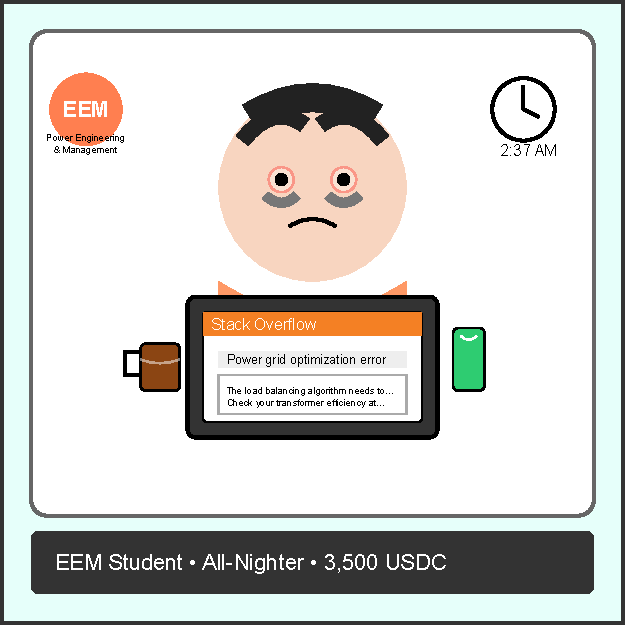
\includegraphics[width=\textwidth]{NFTs/nft-eem-stackoverflow.pdf}
  \end{minipage}
  \hfill
  \begin{minipage}{0.3\textwidth}
    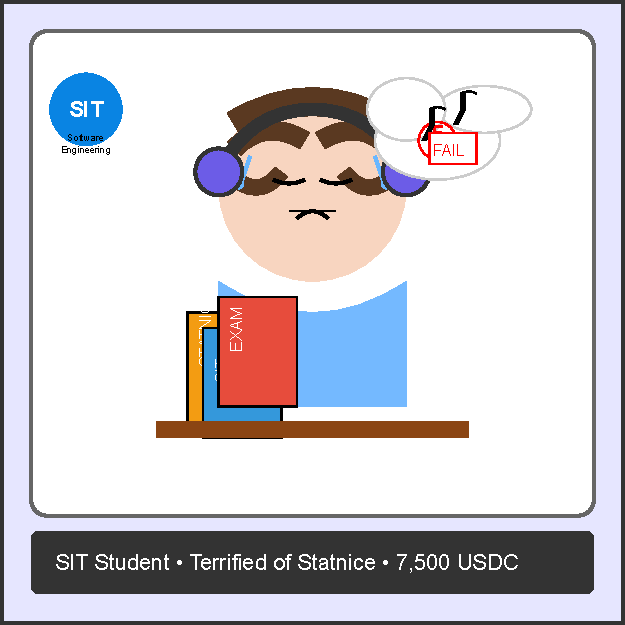
\includegraphics[width=\textwidth]{NFTs/nft-sit-dreaming.pdf}
  \end{minipage}
  \hfill
  \begin{minipage}{0.3\textwidth}
    
\includegraphics[width=\textwidth]{NFTs/nft-uek-power-napper.pdf}
  \end{minipage}
\end{figure}

This time, the marketplace has become more resilient. The SimpleDEX now has a much larger liquidity pool containing 100 ETH and 200,000 USDC, making direct price manipulation much more difficult. At the current exchange rate of 1 ETH = 2,000 USDC, the total value of all NFTs is approximately 8 ETH. As a student, you only have 3 ETH to your name (and no USDC). Buying all three NFTs legitimately is impossible with your current funds. However, you have a secret weapon: Flash Loans! For this challenge, you can use the Flash Loan Provider, which has a pool of 200,000 USDC available for flash loans. The provider charges a minimal fee of just 0.01\% (1 basis point) on all loans.

\medskip
\noindent
\textbf{Your Mission:} Acquire all three FEL Student NFTs despite your limited resources.

Files that are relevant for this challenge:
\begin{itemize}
\item test/\textbf{FoolTheOracle02.js}: The test file where you should code your solution.
\item contracts/\textbf{FlashLoanProvider.sol}: The ERC-3156 compliant flash loan provider with 200,000 USDC.
\item contracts/\textbf{FlashLoanReceiver.sol}: Template for creating a flash loan exploit contract.
\item contracts/\textbf{SimpleDEX.sol}: The DEX with increased liquidity (100 ETH, 200,000 USDC).
\item contracts/\textbf{FELStudentNFT.sol}: The NFT collection.
\item contracts/\textbf{NFTMarketplace.sol}: The marketplace using SimpleDEX as price oracle.
\item contracts/\textbf{USDCToken.sol}: An ERC20 token representing simplified version of USDC.
\end{itemize}

\noindent
Code your solution in the \texttt{test/FoolTheOracle02.js} file and the \\ \texttt{contracts/FlashLoanReceiver.sol} file. Use only the player account. Verify your solution by running the following command:

\begin{minted}[bgcolor=gray!5, fontsize=\footnotesize]{bash}
  $ npm run oracle02
\end{minted}

\end{document}
